%!TEX root = report.tex

\chapter{Finite Element Analysis} % (fold)
\label{cha:finite_element_analysis}
This section gives a basic introduction to the Finite Element Method (FEM) for structural mechanics, and describes the different stages of finite element analysis (FEA). It also presents the software programs that are used in the current analysis workflow at Andritz.

\section{Finite Element Method for Structural Mechanics} % (fold)
\label{sec:finite_element_method_in_structural_mechanics}
The finite element method is technique for finding the approximate solution of differential equations. The differential equations are mathematical models that arise from various physical phenomena, such as heat conduction, electromagnetism and fluid dynamics, but the focus of this thesis is on structural mechanics. The structure, where the differential equations hold, is divided into elements, which in turn consist of $N$ nodes. The nodes are the points where the solution is calculated, and at each node there are usually three spatial degrees of freedom, therefore the total number of degrees of freedom are $3\times N$.~\cite[p.~1--4]{ottossen92}

In structural mechanics the deformation and stresses are calculated for structural objects that are subject to loads (body and surface forces, thermal loads etc.). Two important quantities to mention are stresses and strains. Stresses are the internal forces in a structure that are reactions to the load that is applied to the structure, whereas strain is a measure of the deformation or displacement.~\cite[p.~235ff.]{ottossen92}. The \textit{constitutive relation} describes how stress and strain relate to each other. For linear elasticity Hooke's law, $\sigma=E\varepsilon$, describes the relation, where $\sigma$ is the stress, $\varepsilon$ is the strain and $E$ is Young's modulus. Note that there exists several other constitutive relations which are not considered in this thesis~\cite[p.~248]{ottossen92}.

\subsection{Mathematical Description} % (fold)
\label{sub:mathematical_description}
% TODO: Write generally about weak (p. 56) and strong form (p.51) and relate it to the weak and strong form of solid mechanics. Document the theory!
\textit{The content of this section is based on the book Introduction to the Finite Element Method by Niels Ottossen and Hans Petersson~\cite{ottossen92}, for a more detailed description of the material the reader is referred to that source.}

This section describes the FE procedure: how to get from the mathematical model (ie. differential equations) to a system of equations that can be solved with a numerical approach.

Given the stress tensor
\begin{equation}
\label{eq:stress_tensor}
	\mathbf{S} = 
	\begin{bmatrix}
	\sigma_{xx} & \sigma_{xy} & \sigma_{xz} \\
	\sigma_{yx} & \sigma_{yy} & \sigma_{yz} \\
	\sigma_{zx} & \sigma_{zy} & \sigma_{zz}
	\end{bmatrix},
\end{equation}
the stress equilibrium is given by
\begin{equation}
\label{eq:stress_equilibrium}
	\begin{cases}
		\dfrac{\partial \sigma_{xx}}{\partial x} + \dfrac{\partial \sigma_{xy}}{\partial y} + \dfrac{\partial \sigma_{xz}}{\partial z} + b_x = 0 \\
		\dfrac{\partial \sigma_{yx}}{\partial x} + \dfrac{\partial \sigma_{yy}}{\partial y} + \dfrac{\partial \sigma_{yz}}{\partial z} + b_y = 0 \\
		\dfrac{\partial \sigma_{zx}}{\partial x} + \dfrac{\partial \sigma_{zy}}{\partial y} + \dfrac{\partial \sigma_{zz}}{\partial z} + b_z = 0
	\end{cases}
	\Leftrightarrow
	\,\, \widetilde{\nabla}^T \bm{\sigma} + \mathbf{b} = \mathbf{0}
\end{equation}
where $\widetilde{\nabla}^T$ is a differential operator and $\mathbf{b}$ is the body force acting on the structure. The strain kinematic relation is
\begin{equation}
\label{eq:strain_kinematic_relation}
 	\bm{\varepsilon} = \widetilde{\nabla}^T \mathbf{u},
\end{equation} 
where $\mathbf{u}$ is the displacement vector.

The boundary conditions are given by the traction vector $\mathbf{t}$ or a prescribed displacement $\mathbf{u}$ on the surface of the structure:
\begin{equation}
\label{eq:boundary_condition}
	\begin{cases}
 		\mathbf{t} = \mathbf{S}\mathbf{n} = \mathbf{h} & \text{on $S_h$} \\
		\mathbf{u} = \mathbf{g} & \text{on $S_g$}
	\end{cases}
\end{equation}
where $\mathbf{n}$ is the normal vector of the surface. The \textit{strong formulation} of elasticity is given by Equation~\eqref{eq:stress_equilibrium} and \eqref{eq:strain_kinematic_relation} with boundary conditions given by Equation~\eqref{eq:boundary_condition}.

To obtain the weak formulation the standard procedure is to multiply the strong formulation with a weight function $\mathbf{v}$ and then integrate over the volume; the case with Equation~\eqref{eq:stress_equilibrium} yields
\begin{equation}
	\int_V \mathbf{v} \widetilde{\nabla}^T \bm{\sigma} \,\mathrm{d}V + \int_V \mathbf{v} \mathbf{b} \,\mathrm{d}V = \bm{0}.
\end{equation}
Using Green's theorem and the boundary condition in Equation~\eqref{eq:boundary_condition} the \textit{weak formulation} of the stress equilibrium equation is obtained
\begin{equation}
	\label{eq:weak_formulation}
	\int_V \left(\widetilde{\nabla} \mathbf{v}\right)^T \bm{\sigma} \,\mathrm{d}V = \int_S \mathbf{v}^T \mathbf{t} \,\mathrm{d}S + \int_V \mathbf{v}^T \mathbf{b} \,\mathrm{d}V.
\end{equation}

The FE formulation is based on the weak formulation, where the continuous displacement vector in the weak formulation is approximated by
\begin{equation}
	\label{eq:displacement_approximation}
	\mathbf{u} = \mathbf{N}\mathbf{a}
\end{equation}
where $\mathbf{N}$ is a \textit{shape function matrix} and $\mathbf{a}$ is the nodal displacement vector. Using the same approximation for the weight function yields
\begin{equation}
	\label{eq:weight_function_approximation}
	\mathbf{v} = \mathbf{N}\mathbf{c},
\end{equation}
where $\mathbf{c}$ is an arbitrary vector. If Equation~\eqref{eq:weight_function_approximation} is used in the weak formulation~\eqref{eq:weak_formulation}, the following expression is obtained
\begin{equation}
	\int_V \left(\widetilde{\nabla} \mathbf{N}\right)^T \bm{\sigma} \,\mathrm{d}V = \int_S \mathbf{N}^T \mathbf{t} \,\mathrm{d}S + \int_V \mathbf{N}^T \mathbf{b} \,\mathrm{d}V.
\end{equation}
Using the constitutive relation between stress and strain (in this case Hooke's law)
\begin{equation}
	\label{eq:hookes_law}
	\bm{\sigma} = \mathbf{D}\bm{\varepsilon},
\end{equation}
where $\mathbf{D}$ is the constitutive matrix and Equation~\ref{eq:strain_kinematic_relation}, the final FE formulation is obtained
\begin{equation}
	\label{eq:fe_formualtion}
	\mathbf{K}\mathbf{a} = \mathbf{f}.
\end{equation}
$\mathbf{K}$ is the stiffness matrix given by
\begin{equation}
	\mathbf{K} = \int_V \left(\widetilde{\nabla} \mathbf{N}\right)^T \mathbf{D} \left(\widetilde{\nabla} \mathbf{N}\right) \,\mathrm{d}V,
\end{equation}
and $\mathbf{f}$ is the force vector that is composed of the body forces, boundary conditions and the initial strain.

The system of equations that~\eqref{eq:fe_formualtion} represent is the system that is solved by the solver and the solution $\mathbf{a}$ is the approximation of the displacement vector $\mathbf{u}$. The size (ie. the number of unknowns) of the system is $3\times N$, where $N$ is the number of nodes in the mesh.
% subsection mathematical_description (end)

\subsection{Elements} % (fold)
\label{sub:elements}
A principal feature of FEM is that the unknown function (in this case the displacement) is approximated by dividing the geometry into a finite number of elements, which enables the method to approximate the unknown function on complex geometries. How these elements are constructed depend on the geometry and the problem definition. This section presents simple two- and three-dimensional elements that are common in FEA.

The unknown is approximated by a polynomial, and the simplest element is the linear one-dimensional element. If a one-dimensional geometry is divided into $N-1$ elements with $N$ nodes, the unknown is approximated on element $i$ by a \textit{shape functions} given by
\begin{equation}
	\label{eq:shape_function}
	\varphi_i = 
	\begin{cases}
		(x-x_{i-1})/h_i & \text{if $x_{i-1} \leq x \leq x_i$} \\
		(x_{i+1}-x)/h_{i+1} & \text{if $x_i < x \leq x_{i+1}$} \\
		0 & \text{else}
	\end{cases}
	,
\end{equation}
where $h_i$ is the length of the element. The approximation over the entire geometry is then given by
\begin{equation}
	\label{eq:linear_approximation}
	u = \sum_{i=0}^n \alpha_i \varphi_i(x),
\end{equation}
where $\alpha_i$ is a constant parameter (see Fig.~\ref{fig:shape_function}).
\begin{figure}[t]
	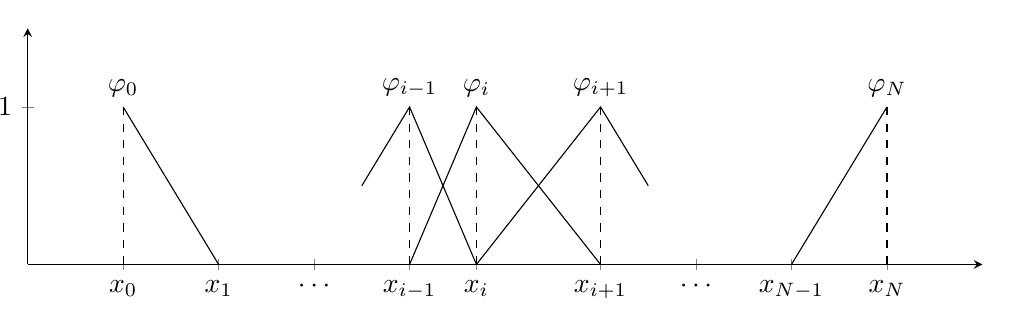
\begin{tikzpicture}[
	baseline,
	trim axis left,
	]
		\begin{axis}[
			width=1\textwidth,
			height=3cm,
			xmin=0,xmax=10,
			xtick={1,2,3,4,4.7,6,7,8,9},
			xticklabels={$x_0$,$x_1$,$\cdots$,$x_{i-1}$,$x_i$,$x_{i+1}$,$\cdots$,$x_{N-1}$,$x_N$},
			ymin=0,ymax=1.5,
			ytick={1},
			axis x line=bottom,
			axis y line=left,
			scale only axis,
		]
			\draw (axis cs:1,1) -- (axis cs:2,0);
			\draw (axis cs:4,0) -- (axis cs:4.7,1) -- (axis cs:6,0);
			\draw (axis cs:8,0) -- (axis cs:9,1);
			\draw (axis cs:3.5,.5) -- (axis cs:4,1) -- (axis cs:4.7,0);
			\draw (axis cs:4.7,0) -- (axis cs:6,1) -- (axis cs:6.5,.5);
			\draw[dashed] (axis cs:1,1) -- (axis cs:1,0);
			\draw[dashed] (axis cs:6,1) -- (axis cs:6,0);
			\draw[dashed] (axis cs:4.7,1) -- (axis cs:4.7,0);
			\draw[dashed] (axis cs:9,1) -- (axis cs:9,0);
			\draw[dashed] (axis cs:4,1) -- (axis cs:4,0);
			\node[above] at (axis cs:4,1) {$\varphi_{i-1}$};
			\node[above] at (axis cs:6,1) {$\varphi_{i+1}$};
			\node[above] at (axis cs:1,1) {$\varphi_0$};
			\node[above] at (axis cs:4.7,1) {$\varphi_i$};
			\node[above] at (axis cs:9,1) {$\varphi_N$};
		\end{axis}
	\end{tikzpicture}
	\caption{A one-dimensional mesh and the corresponding linear shape functions.}
	\label{fig:shape_function}
\end{figure}
Instead of linear interpolation between the nodes, a quadratic element can be defined by introducing a nodal point in the middle of the element.~\cite[p.~1ff.]{larsson13}

Two- and three-dimensional elements are constructed by the same principle as described above, although the  mathematical description is more involved. A three-node triangular element is shown in Figure~\ref{subfig:triangular_element}, Figure~\ref{subfig:rectangular_element} shows a four-node rectangular element, Figure~\ref{subfig:tetrahedral_element} shows a four-node tetrahedral element and Figure~\ref{subfig:hexahedral_element} Higher order elements can be constructed by adding nodes on the mid-points of the elements, just as with the one-dimensional elements.~\cite[p.~118ff.]{ottossen92}
\begin{figure}[t]
	\begin{subfigure}{.5\textwidth}
	\begin{center}
		\begin{tikzpicture}[baseline]
			\begin{axis}[
				axis x line=bottom,
				axis y line=left,
				ticks=none,
				xmin=0,xmax=10,
				ymin=0,ymax=10,
				width=1\textwidth,
				xlabel=$x$, ylabel=$y$,
				every axis x label/.style={
				    at={(ticklabel* cs:1.05)},
				    anchor=west,
				},
				every axis y label/.style={
				    at={(ticklabel* cs:1.05)},
				    anchor=south,
				},
			]
				\draw (axis cs:2,2) -- (axis cs:6,8) -- (axis cs:8,3) -- (axis cs:2,2);
				\draw[fill] (axis cs:2,2) circle [radius=0.1];
				\node[below] at (axis cs:2,2) {$(x_1,y_1)$};
				\draw[fill] (axis cs:6,8) circle [radius=0.1];
				\node[above] at (axis cs:6,8) {$(x_2,y_2)$};
				\draw[fill] (axis cs:8,3) circle [radius=0.1];
				\node[below] at (axis cs:8,3) {$(x_3,y_3)$};
			\end{axis}
		\end{tikzpicture}
		\caption{Three-node triangular element.}
		\label{subfig:triangular_element}
	\end{center}
	\end{subfigure}
	\begin{subfigure}{.5\textwidth}
	\begin{center}
		\begin{tikzpicture}[baseline]
			\begin{axis}[
				axis x line=bottom,
				axis y line=left,
				ticks=none,
				xmin=0,xmax=10,
				ymin=0,ymax=10,
				width=1\textwidth,
				xlabel=$x$, ylabel=$y$,
				every axis x label/.style={
				    at={(ticklabel* cs:1.05)},
				    anchor=west,
				},
				every axis y label/.style={
				    at={(ticklabel* cs:1.05)},
				    anchor=south,
				},
			]
				\draw (axis cs:2,2) -- (axis cs:2,8) -- (axis cs:8,8) -- (axis cs:8,2) -- (axis cs:2,2);
				\draw[fill] (axis cs:2,2) circle [radius=0.1];
				\node[below] at (axis cs:2,2) {$(x_1,y_1)$};
				\draw[fill] (axis cs:2,8) circle [radius=0.1];
				\node[above] at (axis cs:2,8) {$(x_2,y_2)$};
				\draw[fill] (axis cs:8,8) circle [radius=0.1];
				\node[above] at (axis cs:8,8) {$(x_3,y_3)$};
				\draw[fill] (axis cs:8,2) circle [radius=0.1];
				\node[below] at (axis cs:8,2) {$(x_4,y_4)$};
			\end{axis}
		\end{tikzpicture}
		\caption{Four-node rectangular element.}
		\label{subfig:rectangular_element}
	\end{center}
	\end{subfigure}%
	\\
	\begin{subfigure}{.5\textwidth}
	\begin{center}
		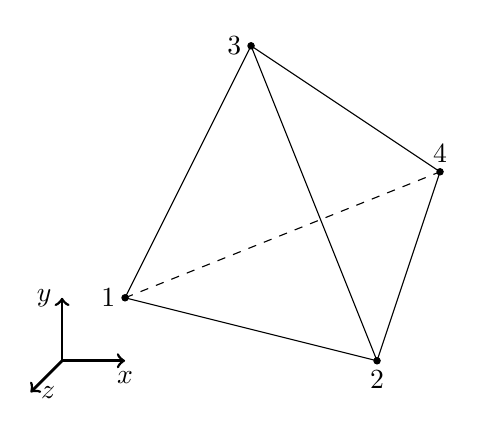
\begin{tikzpicture}[baseline,scale=.8]
			\draw [line width=1,->] (0,0) -- (1,0) node [below] {$x$};
			\draw [line width=1,->] (0,0) -- (0,1) node [left] {$y$};
			\draw [line width=1,->] (0,0) -- (-.5,-.5) node [right] {$z$};
			\draw (1,1) -- (3,5) -- (6,3) -- (5,0) -- (1,1);
			\draw (3,5) -- (5,0);
			\draw[dashed] (1,1) -- (6,3);
			\draw[fill] (1,1) circle [radius=0.05] node[left] {$1$};
			\draw[fill] (5,0) circle [radius=0.05] node[below] {$2$};
			\draw[fill] (3,5) circle [radius=0.05] node[left] {$3$};
			\draw[fill] (6,3) circle [radius=0.05] node[above] {$4$};
		\end{tikzpicture}
		\caption{Four-node tetrahedral element.}
		\label{subfig:tetrahedral_element}
	\end{center}
	\end{subfigure}
	\begin{subfigure}{.5\textwidth}
	\begin{center}
		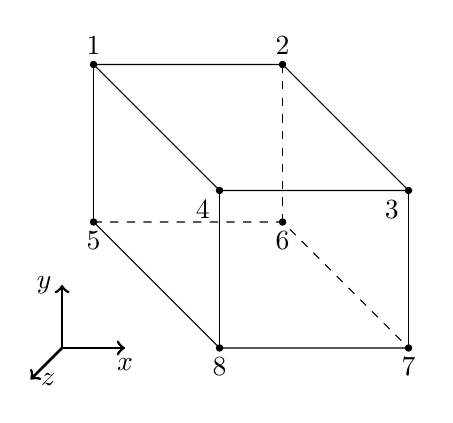
\begin{tikzpicture}[baseline,scale=.8]
			\draw [line width=1,->] (0,0) -- (1,0) node [below] {$x$};
			\draw [line width=1,->] (0,0) -- (0,1) node [left] {$y$};
			\draw [line width=1,->] (0,0) -- (-.5,-.5) node [right] {$z$};
			% \draw (1,4) node[below] {$1$} -- (1,6) node[below] {$2$} -- (4,6) node[below] {$3$} -- (6,4) node[below] {$4$} -- (6,2) node[below] {$5$} -- (3,2) node[below] {$6$} -- (1,4) -- (1,6) -- (3,4) node[below] {$7$} -- (6,4) -- (3,4) -- (3,2);
			\draw (.5,4.5) node[above] {$1$} -- (3.5,4.5) node[above] {$2$} -- (5.5,2.5) node[below left] {$3$} -- (2.5,2.5) node[below left] {$4$} -- (.5,4.5);
			\draw[dashed] (.5,2) node[below] {$5$} -- (3.5,2) node[below] {$6$} -- (5.5,0) node[below] {$7$};
			\draw (5.5,0) -- (2.5,0) node[below] {$8$} -- (.5,2);
			\draw (.5,4.5) -- (.5,2);
			\draw (2.5,2.5) -- (2.5,0);
			\draw (5.5,2.5) -- (5.5,0);
			\draw[dashed] (3.5,4.5) -- (3.5,2);
			\draw[fill] (.5,4.5) circle [radius=0.05];
			\draw[fill] (3.5,4.5) circle [radius=0.05];
			\draw[fill] (5.5,2.5) circle [radius=0.05];
			\draw[fill] (2.5,2.5) circle [radius=0.05];
			\draw[fill] (.5,2) circle [radius=0.05];
			\draw[fill] (3.5,2) circle [radius=0.05];
			\draw[fill] (5.5,0) circle [radius=0.05];
			\draw[fill] (2.5,0) circle [radius=0.05];
		\end{tikzpicture}
		\caption{Eight-node hexahedral element.}
		\label{subfig:hexahedral_element}
	\end{center}
	\end{subfigure}%
	\caption{Two- and three-dimensional elements.}
	\label{fig:elements}
\end{figure}
% subsubsection elements (end)

% \subsection{Boundary Conditions} % (fold)
% \label{sub:boundary_condidtions}
% Describe different types of bc's.
% % subsubsection boundary_condidtions (end)

% \subsection{Load Cases} % (fold)
% \label{sub:load_cases}
% Maybe not necessary
% % subsubsection load_cases (end)

\subsection{Contacts} % (fold)
\label{sub:contacts}
Describe non-linearity, meshing technique etc.
The differential equations presented in Section~\ref{sub:mathematical_description} are linear, and are thus easy to handle with the FEM. However, there exists many structural problems where the governing differential equations are non-linear. Non-linear differential equations in structural mechanics can relate to material, geometric, force and kinematic non-linearities; and the focus of this section is on kinematic non-linearities from contact problems. Since this thesis does not investigate the solution process, this section does not delve into to the topic, but merely mentions it and how the FE model should be prepared if contacts are present in the analysis.

Contact problems occur when two or more structures come in contact with each other during the simulation. This means that the boundary condition prescribing the displacement depends on the deformations. This is handled in by introducing constraint equations to the system of equations. Generally, contacts can involve friction, large displacements and inelastic behaviour. For static analyses it is important to set boundary conditions such that no rigid-body motion is possible.~\cite[p.~549ff.]{bhatti06}
% subsubsection contacts (end)

% subsection finite_element_method_in_structural_mechanics (end)

\section{FEA Workflow} % (fold)
\label{sec:fea_workflow}
The FEA consist of three phases: pre-processing, solution and post-processing; this section describes these phases.

\subsection{Pre-Processing} % (fold)
\label{sub:pre_processing}
When a structure has been designed, the CAD model needs to be analysed to determine if the desired performance qualifications are reached. The first step is to translate the CAD model to an FE model, this is called pre-processing. The FE model is a model that is prepared, meshed and have the appropriate properties assigned to it.

% Clean: FEA book p. 181-191
Ideally, the CAD model built by the design team is usable for finite element analysis without having to alter the model. However, this is often not the case, since it often exists features that are problematic from an analysis viewpoint. Therefore, it is necessary to make simplifications to the model in order to create a mesh of the model. Design features that complicate automatic meshing are short edges, sliver faces, small holes, fillets, chamfers etc., and it is necessary to clean the model of these features to enable the automesher to mesh the model. This cleaning process can be both tedious and difficult since it may exist a lot of features, and even if a disadvantageous feature is found it may be difficult to remove it; the cleaning process can therefore be very time consuming. It is also important to mention that the simplifications that are performed should not influence the structural capabilities of the model, this could be difficult to assess, but as long as the simplifications are local and not in areas of interest the structural capabilities should not be affected.~\cite[p.~181--191]{adams99}

% Meshing
When the model is clean, the next step is to mesh the model. Whether the model is meshed automatically or manually and with shell elements or tetrahedrons, the process is an essential step of the analysis. The focus of this thesis is on automeshing with tetrahedrons (for 3D models) and triangles (for 2D models). Automeshing is a simple and efficient technique to create a discrete FE model of the CAD model. Depending on which automesher that is used different settings are available, but the user should generally consider the maximum and minimum elements size, element growth rate and local mesh refinements. The goal is to create a mesh that captures the structural features of the model with as few elements as possible. Even though the automesher could create the mesh in a fast and convenient way, it is no guarantee that the mesh is sufficiently refined. Therefore, considerable thought should be spent on where local mesh refinements are necessary, how small elements are needed and how large elements are excepted. It is also important to mention that it is an absolute necessity that the model is clean, otherwise the automesher will most likely fail to create a mesh.~\cite[p.~251-255]{adams99}

Part of the pre-process is also to define the boundary conditions that influence the model. There exist two groups of boundary conditions: constraints that prohibits the model from moving in the specified spatial degrees of freedom, and loads such as forces, moments and temperature. How the boundary conditions are defined and which types that are used are often not straightforward, and an important part of the analysis.~\cite[p.~263]{adams99}

Before the FE model can be solved the material properties of the model needs to be specified.

It is probably obvious that this part of the analysis can be very time consuming, and to obtain a solution it is of paramount importance that the FE model is created correctly, with sufficient details of the original model and that boundary conditions are properly defined.
% subsubsection pre_processing (end)

\subsection{Solution} % (fold)
\label{sub:solution}
When the FE model is created, the next step is to solve the model to obtain the results. This step is mainly executed by the computer, the only effort from the user is setting the correct solver parameters. Which parameters that can be specified is highly dependent on which solver is used. The execution time depends on how large the FE model is (number degrees of freedom) and what solution type is used (non-linear solutions are more demanding).

When the solver is finished it is important to evaluate the results and the solver output to establish if the solution is reasonable and if the results are accurate. To determine if the mesh is sufficiently refined the convergence should be checked, and to check that the boundary conditions are properly defined the resultant forces on the model could be compared with the specified loads.~\cite[p.~303-324]{adams99}
% subsubsection solution (end)

\subsection{Post-Processing} % (fold)
\label{sub:post_processing}
The first step of the post-processing is to visualise the results (displacement, stress, etc.) to determine if the solution is reasonable. If the solution is reasonable the FE model can be considered to be adequate. The next step is to visualise the specific results that are the goal of the analysis. Even if this step is not very technical, it is important to analyse the results to determine if the results can be trusted.
% subsubsection post_processing (end)

% section fea_workflow (end)

\section{FEA Software Packages} % (fold)
\label{sec:fea_software_packages}
During the development of the FEM, lots of different software programs have been developed. This section describes the software packages that are relevant for this thesis, based on the software packages that are used at Andritz.

\subsection{Siemens NX} % (fold)
\label{sub:siemens_nx}
NX\texttrademark{} is a software developed by Siemens PLM Software that supports every aspect of product development (i.e. design, analysis and manufacturing)~\cite{siemensnx}. NX is a licensed software where the features that are provided is based on which license the user has purchased. This section describes a subset of the functionality provided by NX that is relevant for this thesis. and the focus is on the tools to clean the model (called Synchronous Modelling  tools) and the FEA application (called Advanced Simulation).~\cite[p.~36ff.]{goncharov14}

The synchronous modelling tools that are provided by NX are very efficient and powerful to use during the cleaning process. Synchronous modelling extends the regular parametric modelling approach that is used in CAD with more intuitive and direct modelling tools. The tools that are most commonly used are: \textit{Move Face}, \textit{Delete Face}, \textit{Make Coplanar}, \textit{Pull Face} etc., for a description of these tools see~\cite{goncharov14}. The main advantage of these tools is that the model can be changed without having access to the or making changes to the original history-tree of the commands that created the model.

NX Advanced Simulation provides the entire CAE workflow with pre- and post-processing and solver environment. It is also tightly integrated with the CAD application of NX, enabling a fast and efficient analysis process. The meshing capabilities that Advanced Simulation provides are the usual 3D and 2D automeshers as well as more exotic elements for specific applications. The simulation environment can be integrated with several of the most common solvers such as NX Nastran, Abaqus and Ansys.
% subsection siemens_nx (end)

\subsection{Salomé Platform} % (fold)
\label{sec:salom_platform}
Salomé is a free software platform (distributed under GNU LGPL~\cite{lgpl}) for numerical simulation. Salomé strives to provide a framework where the entire workflow of a numerical simulation (described in Sec.~\ref{sub:pre_processing}-\ref{sub:post_processing}) can take place. The platform consists of different modules that can be used for pre- and post-processing, which are presented under the same GUI (graphical user interface).~\cite{ribes07} 

\subsubsection{Geometry Module} % (fold)
\label{ssub:geometry_module}
The \textit{Geometry} module provides basic functionality to import CAD models and prepare them for numerical simulation. Common tasks that are carried out in this module is to create \textit{groups} and \textit{partition} objects.

A group in Geometry is a collection of geometrical objects (solids, faces, edges or vertices), which is given a common name and can be referenced by that name from other modules. Groups are used for three different purposes: local mesh refinement, boundary conditions and contact surfaces.

To be able to control the automeshing it is useful to define patches on the model where local mesh refinements are necessary to get the solution to converge. A patch is a group of faces or edges that should be better resolved. Any geometrical object of the model that is the subject of a boundary condition should also be defined as a group. If two objects are in contact, and a contact simulation is required, the contact surfaces should be defined as groups.

The partition function connects solid objects and creates a single solid, but the contact face will still remain between the objects. This function is mainly used when a conformal mesh has to be created for a contact simulation.~\cite{salomedoc}
% subsubsection geometry_module (end)

\subsubsection{Mesh Module} % (fold)
\label{ssub:mesh_module}
When a model has been imported to Geometry and and the groups are defined, the \textit{Mesh} module can mesh the model. Mesh provides the most common elements and several different algorithms for mesh generation are available, resulting in a very extensive library of functions.

To mesh an object with the Mesh module first an object from Geometry is selected, then an algorithm is selected and finally an hypothesis is created. The hypothesis represent the parameters that the algorithm use to create the mesh, depending on the algorithm different parameter values are specified in the hypothesis. Since there exist several algorithms in Mesh, this section only describes the \textit{NETGEN} algorithm and the \textit{Projection} algorithm.

The NETGEN algorithm~\cite{netgen} is an automesher that can be used for creating 3D tetrahedral meshes and 2D triangular and quadrilateral meshes. The hypothesis for the NETGEN algorithm specifies
\begin{itemize}
	\item the maximum and minimum element size, 
	\item if second order elements should be used,
	\item growth rate,
	\item the possibility to specify the number of elements based on surface curvature, and
	\item local refinements on specified groups. 
\end{itemize}

The projection algorithm creates a mesh of an object by projecting the mesh of another object. This algorithm is especially used when conformal meshes are desirable.

The mesh module supports, just as the Geometry module, the creation of groups. This feature is specifically useful when a specific part of the mesh needs to be referenced or exported.

\subsubsection{Contact Mesh} % (fold)
\label{ssub:contact_mesh}
If the model contains contacts, it can be necessary to have matching meshes at the contact surface. A matching mesh means that the mesh of the two objects in contact have nodes at the same place at the contact surface. In Salomé there are several ways to obtain a mesh with matching element nodes, here follows a description using the Projection algorithm.

\begin{figure}[t]
	\begin{subfigure}{.35\textwidth}
		\begin{center}
			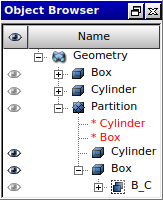
\includegraphics{boxcyl/GeomOB}
		\end{center}
		\caption{Object browser}
		\label{subfig:boxcylgeomob}
	\end{subfigure}
	\begin{subfigure}{.7\textwidth}
		\begin{center}
			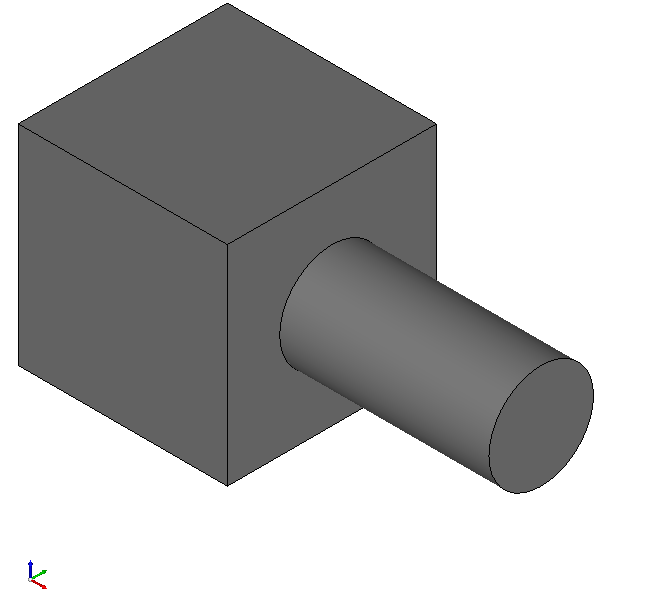
\includegraphics[trim=10 80 50 0,clip,scale=.5]{boxcyl/Geom}
		\end{center}
		\caption{A box and a cylinder in contact.}
		\label{subfig:boxcylgeom}
	\end{subfigure}
	\caption{A simple example demonstrating how a contact mesh can be created in Salomé.}
	\label{fig:boxcylgeom}
\end{figure}

Consider the box and cylinder in Figure~\ref{fig:boxcylgeom}. To create a matching mesh at the contact surface between the box and the element the following steps are required:
\begin{enumerate}
	\item Create a partition of the box and cylinder.
	\item Under the partition create one group containing the box and one containing the cylinder.
	\item Create a sub-group of the contact surface under either box or cylinder (see group \texttt{B\_C} in Fig.~\ref{subfig:boxcylgeomob}).
	\item Mesh the box and cylinder group under the partition separately.
	\item Create a sub-mesh under \texttt{Box} using the Projection algorithm on the contact surface.
\end{enumerate}
The resulting mesh and the Object Browser is depicted in Figure~\ref{fig:boxcylmesh}.

\begin{figure}[t]
	\begin{subfigure}{.35\textwidth}
		\begin{center}
			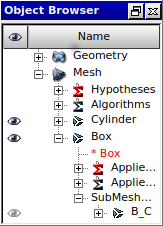
\includegraphics{boxcyl/MeshOB}
		\end{center}
		\caption{Object browser}
		\label{subfig:boxcylmeshob}
	\end{subfigure}
	\begin{subfigure}{.7\textwidth}
		\begin{center}
			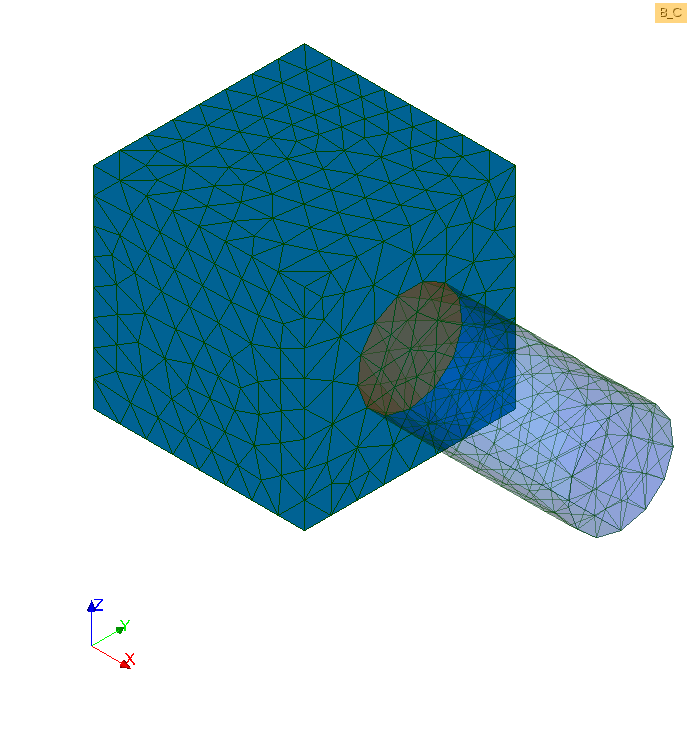
\includegraphics[trim=80 170 10 20,clip,scale=.45]{boxcyl/Mesh}
		\end{center}
		\caption{The contact mesh.}
		\label{subfig:boxcylmesh}
	\end{subfigure}
	\caption{An example of a contact mesh created in Salomé.}
	\label{fig:boxcylmesh}
\end{figure}

% subsubsection contact_mesh (end)
% subsubsection mesh_module (end)

\subsubsection{ParaVis Module} % (fold)
\label{ssub:paravis_module}
The ParaVis module is based on ParaView an open source platform for data analysis and visualisation. Suffice to say that all the functionality needed to visualise the results in a structural analysis is provided.
% subsubsection paravis_module (end)

\subsubsection{Application Programming Interface (API)} % (fold)
\label{ssub:application_programming_interface_}
A very advantageous feature of Salomé and the modules that have been described is that the functionality provided by the GUI also is available through an API, enabling the user to write scripts that execute functions automatically.

An API is a framework of functions for building software applications. Using the API a developer can efficiently create software that perform specific tasks by using the functionality provided by the API. The documentation of the API describes which functions that are available and what each functions does.

Salomé's API is based on the Python programming language and the Salomé GUI includes a Python console, by which the user can execute scripts that utilise the API. There exist a specific API for each module and these can work together within the same script, therefore it is possible to write a script that first import a model to Geometry where groups are created, then the script can select an algorithm and create a hypothesis, and finally the script can update the GUI.

Figure~\ref{fig:salome} gives a simplified view of how the different modules of the Salomé platform interact with each other and with other software programs.

\begin{figure}[t]
	\begin{center}
		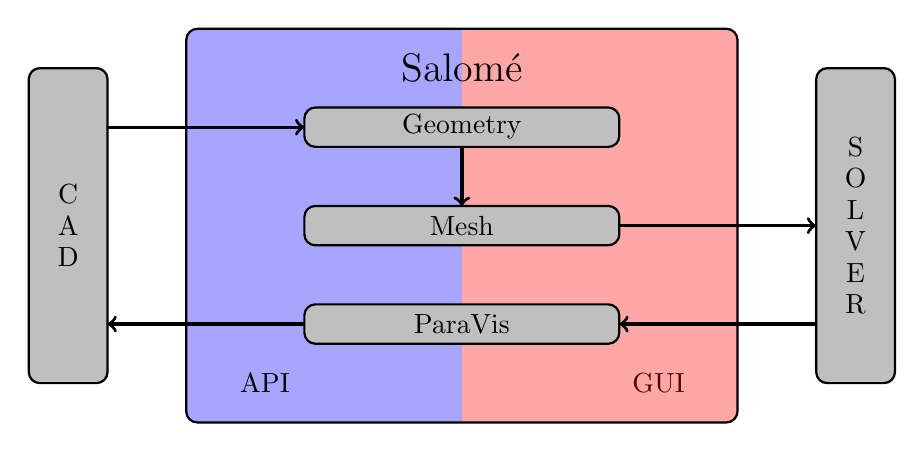
\begin{tikzpicture}
			% CAD
			\draw[rounded corners,fill,lightgray] (0.5,1) -- (1,1) -- (1,5) -- (0,5) -- (0,1) -- (0.5,1);
			\draw[rounded corners,thick] (0.5,1) -- (1,1) -- (1,5) -- (0,5) -- (0,1) -- (0.5,1);
			\node at (.5,3.4) {C};
			\node at (.5,3) {A};
			\node at (.5,2.6) {D};
			% SOLVER
			\draw[rounded corners,fill,lightgray] (10.5,1) -- (11,1) -- (11,5) -- (10,5) -- (10,1) -- (10.5,1);
			\draw[rounded corners,thick] (10.5,1) -- (11,1) -- (11,5) -- (10,5) -- (10,1) -- (10.5,1);
			\node at (10.5,4) 	{S};
			\node at (10.5,3.6) {O};
			\node at (10.5,3.2) {L};
			\node at (10.5,2.8) {V};
			\node at (10.5,2.4) {E};
			\node at (10.5,2) 	{R};
			% GUI
			\draw[fill,blue,rounded corners,opacity=.35] (5.5,.5) -- (2,.5) -- (2,5.5) -- (5.5,5.5);
			\node at (8,1) {GUI};
			% API
			\draw[fill,red,rounded corners,opacity=.35] (5.5,.5) -- (9,.5) -- (9,5.5) -- (5.5,5.5);
			\node at (3,1) {API};
			% SALOME
			\draw[rounded corners,thick] (2,2.5) -- (2,5.5) -- (9,5.5) -- (9,.5) -- (2,.5) -- (2,2.5);
			\node at (5.5,5) {\Large Salomé};
			% Geometry
			\draw[rounded corners,fill,lightgray] (5.5,4) -- ++(2,0) -- ++(0,.5) -- ++(-4,0) -- ++(0,-.5) -- ++(2,0);
			\draw[rounded corners,thick] (5.5,4) -- ++(2,0) -- ++(0,.5) -- ++(-4,0) -- ++(0,-.5) -- ++(2,0);
			\node at (5.5,4.25) {Geometry};
			% Mesh
			\draw[rounded corners,fill,lightgray] (5.5,2.75) -- ++(2,0) -- ++(0,.5) -- ++(-4,0) -- ++(0,-.5) -- ++(2,0);
			\draw[rounded corners,thick] (5.5,2.75) -- ++(2,0) -- ++(0,.5) -- ++(-4,0) -- ++(0,-.5) -- ++(2,0);
			\node at (5.5,3) {Mesh};
			% ParaVis
			\draw[rounded corners,fill,lightgray] (5.5,1.5) -- ++(2,0) -- ++(0,.5) -- ++(-4,0) -- ++(0,-.5) -- ++(2,0);
			\draw[rounded corners,thick] (5.5,1.5) -- ++(2,0) -- ++(0,.5) -- ++(-4,0) -- ++(0,-.5) -- ++(2,0);
			\node at (5.5,1.75) {ParaVis};
			% Arrows
			\draw[->,very thick] (1,4.25) -- (3.5,4.25);
			\draw[<-,very thick] (1,1.75) -- (3.5,1.75);
			\draw[->,very thick] (5.5,4) -- (5.5,3.25);
			\draw[->,very thick] (7.5,3) -- (10,3);
			\draw[->,very thick] (10,1.75) -- (7.5,1.75);
		\end{tikzpicture}
	\end{center}
	\caption{A schematic view of the Salomé platform}
	\label{fig:salome}
\end{figure}

% subsubsection application_programming_interface_ (end)

% subsection salom_platform (end)

\subsection{Code Aster} % (fold)
\label{sub:code_aster}
Code Aster~\cite{codeaster} is an open source FEM software for structural analysis which is developed by EDF (Électricité de France) and distributed under GPL (General Public License)~\cite{gpl}. The software is driven by an input file with commands that that describe the simulation (a COMM file), and a text file describing the mesh (usually a MAIL file). The information the MAIL file needs to contain is the mesh data, that is the nodes and the elements of the mesh, but the file also needs to describe the patches on which the boundary conditions are applied, these patches can be created in the Mesh module as described in Section~\ref{ssub:mesh_module}. The output is text files describing general information about the simulation (errors, warnings, convergence, etc.) and a file containing the results which can be imported to Salomé and visualised with the ParaVis module. 
% subsection code_aster (end)

% section fea_software_packages (end)

% section finite_element_analysis (end)